\documentclass{summarysheet}

\begin{document}


\maketitle{7}{Current and Resistance}

\begin{multicols}{2}

\begin{topicbox}{Current}

%\begin{multicols}{2}
\noindent Current is the motion of charges sustained by an electric field.  
\begin{itemize}
\item Electron current $i_e$ is the rate of flow of electrons.
\item Conventional current $I$ is the rate of flow of charge,
\begin{eqbox}
I = \frac{dQ}{dt}.
\end{eqbox}
\item The current density $J = I/A$, where $A$ is the cross-sectional area of the wire.
\end{itemize}
\begin{center}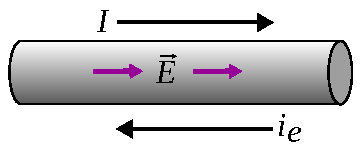
\includegraphics[scale=0.5]{fig_wire.pdf}\end{center}
%\end{multicols}

\end{topicbox}


\begin{topicbox}{Ohm's Law}

\noindent An electric field $E$ in a conductor creates a current density 
\[
J = \sigma E,
\]
where $\sigma$ is the \emph{conductivity} of the material. The \emph{resistivity} of the material is $\rho = 1/\sigma$. The resistance of a conductor of length $L$ is given by
\[
R = \frac{\rho L}{A}.
\]
The unit of resistance is ohms (1 $\Omega = 1$ V/A).

\noindent Ohm’s law says that the current through a conductor is given by
\begin{eqbox}
I = \frac{\Delta V}{R},
\end{eqbox}
where $\Delta V$ is the voltage across the ends of the conductor.
\end{topicbox}




\begin{topicbox}{Kirchhoff's Laws}

\noindent \textbf{Kirchhoff's Junction Law}

\noindent Since charge is conserved, the current into a junction is equal to the current leaving the junction:
\begin{eqbox}
\sum I_\text{in} = \sum I_\text{out}.
\end{eqbox}

\noindent \textbf{Kirchhoff's Loop Law}

\noindent Since energy is conserved, the sum of all voltages in a complete loop in a circuit is zero:
\begin{eqbox}
\Delta V_\text{loop} = \sum_i \Delta V_i = 0.
\end{eqbox}

\noindent The voltage here is $\Delta V = V_\text{downstream} – V_\text{upstream}$, so that
\begin{itemize}
\item For an ideal battery in the negative to positive direction, $\Delta V = +\mathcal{E}$.
\item For an ideal battery in the positive to negative direction, $\Delta V = -\mathcal{E}$.
\item For a resistor, the potential decreases across the resistor in the direction of the current, so $\Delta V = −IR$.
\end{itemize}

\end{topicbox}





\begin{topicbox}{Batteries}

\noindent A battery is a source of potential difference (voltage) $\Delta V_\text{bat}$. This voltage causes an electric field in a connected wire, which establishes a current $I$. The magnitude of the current is determined by Ohm’s law.
\begin{itemize}
\item An ideal battery has a voltage $\Delta V_\text{bat} = \mathcal{E}$.
\item A real battery has internal resistance $r$ and a voltage $\Delta V_\text{bat} = \mathcal{E} - Ir$.
\item The power delivered by a battery is $P_\text{bat} = I\mathcal{E}$.
\end{itemize}
\end{topicbox}









\begin{topicbox}{Resistor Circuits}

\begin{multicols}{2}
\noindent \textbf{Resistors in Series}

\noindent When connected in series, resistors have the same current through them but different voltage $\Delta V_R$. Resistances add to an equivalent resistance:
\begin{eqbox}
R_\text{eq} = R_1 + R_2 + R_3 + \cdots
\end{eqbox}
\begin{center} 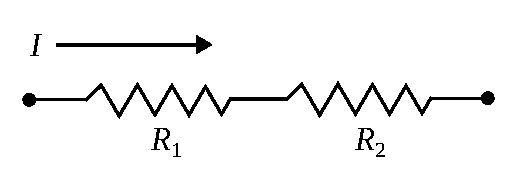
\includegraphics[scale=0.5]{fig_series.pdf} \end{center}

\vspace{0.5in}

\noindent \textbf{Resistors in Parallel}

\noindent When connected in parallel, resistors have the same voltage $\Delta V_R$ but different current. Resistances add in inverse to an equivalent resistance:
\begin{eqbox}
R_\text{eq} = \left( \frac{1}{R_1} + \frac{1}{R_2}  + \frac{1}{R_3} + \cdots \right)^{-1}
\end{eqbox}
\begin{center} 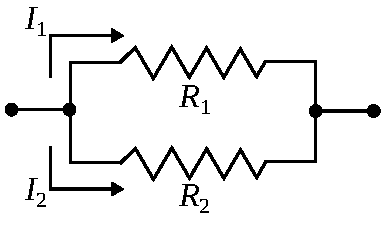
\includegraphics[scale=0.5]{fig_parallel.pdf} \end{center}

\end{multicols}

\noindent \textbf{Power}

\noindent The power dissipated by a resistor is
\begin{eqbox}
P_R = I \Delta V_R = I^2R = \frac{\Delta V_R^2}{R}.
\end{eqbox}

\noindent \textbf{Measuring Current and Voltage}

\begin{itemize}
\item An \emph{ammeter} measures current $I$ in a circuit element. It must be placed in series with the element. An ideal ammeter has zero resistance.
\item A voltmeter measures the voltage $\Delta V$ across a circuit element. It must be placed in parallel with the element. An ideal voltmeter has infinite resistance.
\end{itemize}

\end{topicbox}




\begin{topicbox}{$RC$ Circuits}

\noindent A capacitor can be discharged by connecting it to a resistor, and charged by connecting it to a resistor and battery.
\begin{itemize}
\item Discharging a capacitor:
\begin{eqbox}
Q = Q_0 e^{-t/\tau} \quad \quad \quad I = I_0 e^{-t/\tau}.
\end{eqbox}
\item Charging a capacitor:
\begin{eqbox}
Q = Q_0 \left( 1 - e^{-t/\tau} \right) \quad \quad \quad I = I_0 e^{-t/\tau}.
\end{eqbox}
\end{itemize}

\noindent The time constant $\tau  = RC$ determines how quickly the capacitor is charged and discharged.

\end{topicbox}



\end{multicols}




\makebanner{Electricity and Magnetism}

\end{document}



